\documentclass[aps,twocolumn,secnumarabic,balancelastpage,amsmath,amssymb,nofootinbib,floatfix]{revtex4-1}

\usepackage{graphicx}      % tools for importing graphics
\usepackage[colorlinks=true]{hyperref}  % this package should be added 
\usepackage{dcolumn}% Align table columns on decimal point
\usepackage{bm}% bold math
\usepackage{xcolor}

\newcommand{\kev}{\,{\rm keV}}
\newcommand{\s}{\,{\rm s}}


\begin{document}

\title{Compton Scattering}

\author{Vinh Tran}
\affiliation{Department of Physics and Kavli Institute for Astrophysics and Space Research, Massachusetts Institute of Technology, Cambridge, MA 02139, USA}
\email{vinhtran@mit.edu}

\date{\today}

%%%%%%%%%%%%%%%%%%%%%%%%%%%%%%%%%%%%%%%%%%%%%%%%%%%%%%%%%%%%%%%%%%

\begin{abstract}



\end{abstract}

\maketitle

%%%%%%%%%%%%%%%%%%%%%%%%%%%%%%%%%%%%%%%%%%%%%%%%%%%%%%%%%%%%%%%%%%

\section{Introduction}
\label{sec:intro}




\section{Experiment Setup}
\label{sec:experiment}

\subsection{Apparatus}
\label{sec:apparatus}



\subsection{Data Collection}
\label{sec:data_collection}

\begin{table}
    \centering
    \addtolength{\tabcolsep}{3pt}
    \def\arraystretch{1.5}
    \begin{tabular}{c c c c}
        \hline
        $\theta$ & Counting Time & Total Time & Collection Date \\ [0ex]
         & $[\rm{s}]$ & $[\rm{s}]$ & [YYYY-MM-DD] \\ [1ex]
        \hline\hline

        0 & 964 & 1012 & 2025-03-04 \\
        30 & 1194 & 1224 & 2025-03-04 \\
        60 & 1619 & 1658 & 2025-03-04 \\
        90 & 1856 & 1900 & 2025-03-04 \\
        120 & 1706 & 1736 & 2025-03-04 \\
        15 & 1354 & 1522 & 2025-03-06 \\
        45 & 1333 & 1455 & 2025-03-06 \\
        75 & 1954 & 2058 & 2025-03-06 \\
        105 & 1645 & 1727 & 2025-03-06 \\
        135 & 1341 & 1431 & 2025-03-06 \\
        
        \hline
        
    \end{tabular}
    \caption{}
    \label{tab:data_collection}    
\end{table}


\section{Results}
\label{sec:result}

\begin{figure}
    \centering
    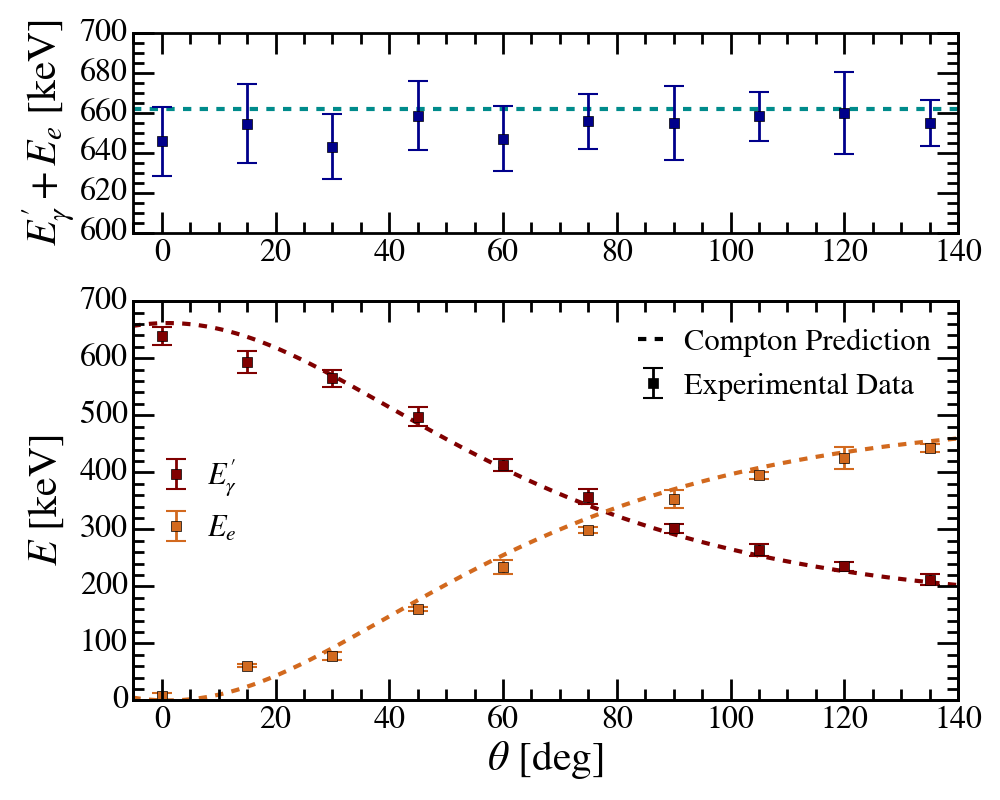
\includegraphics[width=0.49 \textwidth]{Figures/energy_angle_dependency.png}
    \caption{}
    \label{fig:energy_angle_dependency}
\end{figure}

\begin{figure}
    \centering
    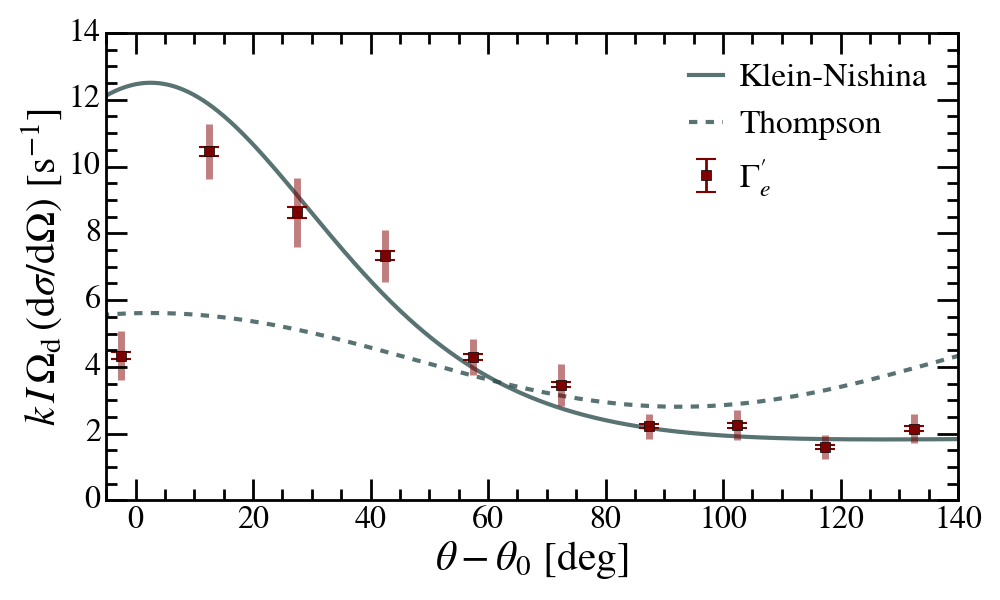
\includegraphics[width=0.49 \textwidth]{Figures/scattering_rate.png}
    \caption{}
    \label{fig:scattering_rate}
\end{figure}


\section{Discussion and Conclusion}
\label{sec:conclusion}




\begin{acknowledgments}

The author thanks his lab partner  Y. Hu for collaboration in the experiment, support in the formatting and structuring of the manuscript. The author also thanks the JLab teaching staffs for their guidance and support, as well as the MIT Physics Department for providing the experimental apparatus.

\end{acknowledgments}

%%%%%%%%%%%%%%%%%%%%%%%%%%%%%%%%%%%%%%%%%%%%%%%%%%%%%%%%%%%%%%%%%%

\bibliography{ref}

%%%%%%%%%%%%%%%%%%%%%%%%%%%%%%%%%%%%%%%%%%%%%%%%%%%%%%%%%%%%%%%%%%

\appendix

\section{Energy Calibration}
\label{app:energy_calibration}

\begin{figure}
    \centering
    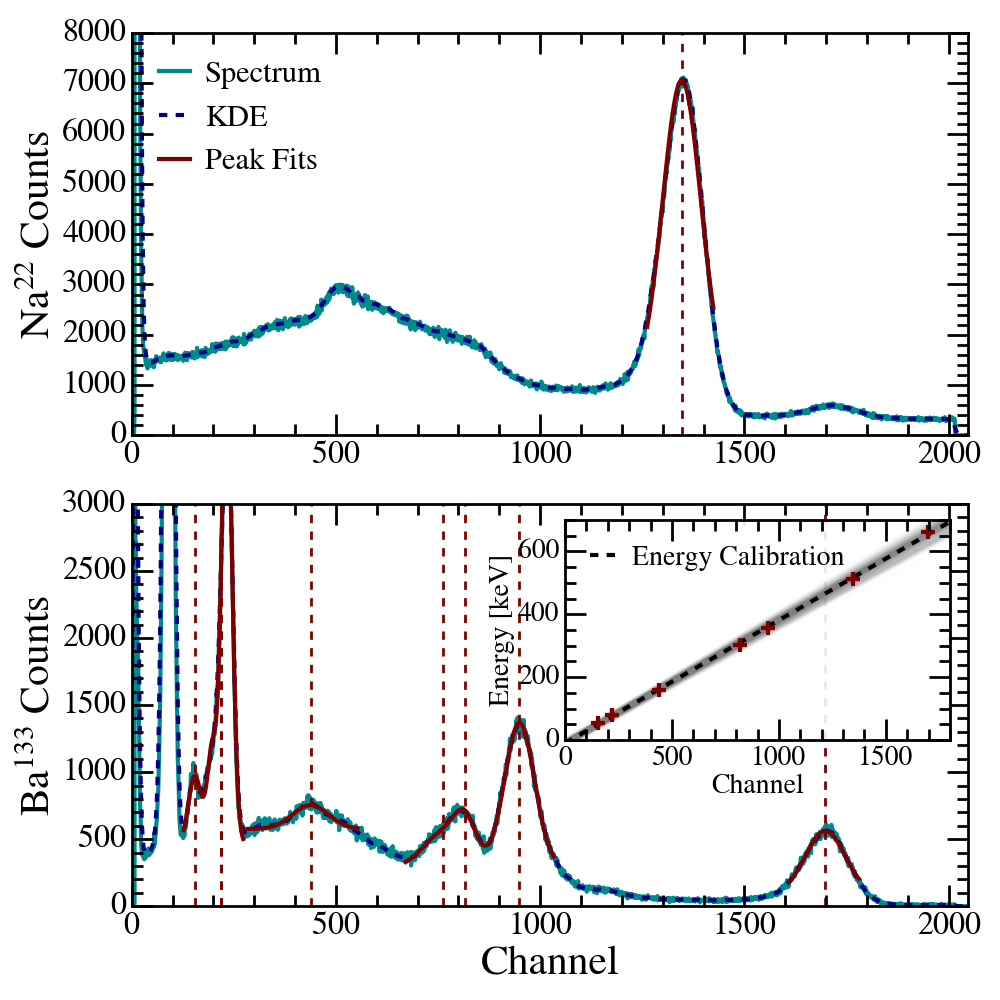
\includegraphics[width=0.49 \textwidth]{Figures/energy_calibration.png}
    \caption{}
    \label{fig:energy_calibration}
\end{figure}

\end{document}